\section{Log Extension} \label{sec:log}
Now we shift our focus towards detecting some types of log misbehavior, namely,
omission attacks but \emph{not} inconsistency attacks.  The design idea is an
extension of our base design, and a prerequisite is that the CT log landscape
is modified to support \emph{SCT cross-logging}.  Cross-logging, in general,
refers to the idea of logging signed statements in other logs to intertwine
them, thus making it more difficult to get away with
misbehavior.  We use the same idea, but apply it to SCTs.  This means that CTRs
can log SFOs rather than certificate chains, thereby making it possible to
detect MMD violations.

\subsection{Design Sketch}
\begin{figure*}
    \centering
    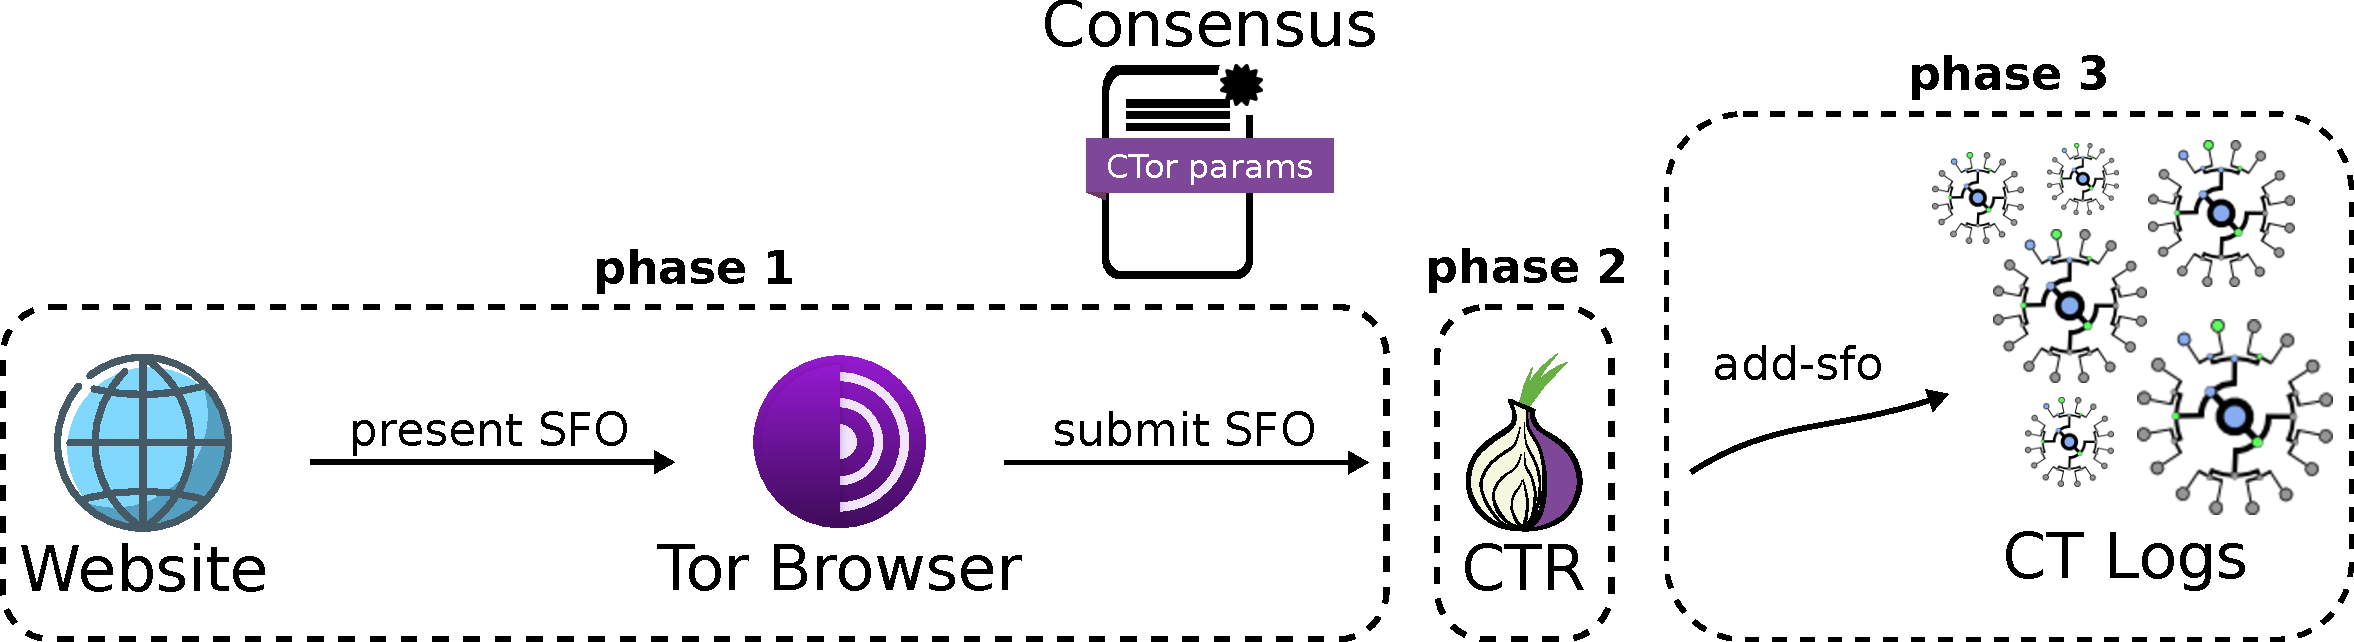
\includegraphics[width=0.85\textwidth]{img/design-log}
    \caption{todo Tobias}
    \label{fig:design-log}
\end{figure*}

%
% Tor consensus
% - No changes
%

%
% Phase 1---Tor browser
% - No changes
%

%
% Phase 2---Storage
% - Updated steps to compute an audit_after timestamp.
%   --> Should we still base on random SCT, or max MMD?
%

%
% Phase 3---Auditing
% - Updated submission endpoint, i.e., submit SFO rather than cert chain
%

%
% Extra-info document
% - Need flushing statistics
%

\subsection{Security Sketch}
%
% MISC notes
% - Network-wide flush, detectable but hard to attribute
% - Requires that the logs extend their APIs to accept SCT cross-logging
%
